
\documentclass{report}

\input{preamble}
\input{macros}
\input{letterfonts}

\title{\Huge{Economia Aziendale}\\Sistemi Informativi Aziendali}
\author{\huge{Caberlotto Giovanni}}
\date{}

\begin{document}

\maketitle
\newpage% or \cleardoublepage
% \pdfbookmark[<level>]{<title>}{<dest>}
\pdfbookmark[section]{\contentsname}{toc}
\tableofcontents
\pagebreak

\chapter{Contabilità Generale e Bilancio} % (fold)
\label{chap:Contabilità Generale e Bilancio}

\section{Contabilità Generale}

% section Contabilità Generale (end)


\section{Bilanci Aziendali e Revisione Legale dei Conti}
\subsection{Il bilancio d'esercizio}
\\
Il bilancio d'esercizio è un documento redatto dagli organi amministrativi al termine del periodo amministrativo, sintetizzando la situazione patrimoniale, finanziaria e il risultato economico dell'azienda. Funge da rendiconto della gestione, offrendo una visione retrospettiva e servendo come strumento di controllo per gli organi amministrativi. Derivante da "rendere conto," il termine "rendiconto" rappresenta un resoconto degli eventi accaduti.
\\
\\
Nel contesto dell'informativa aziendale, il bilancio è cruciale per fornire informazioni essenziali sulla consistenza patrimoniale, andamenti finanziari ed economici. Queste informazioni, storiche o prospettiche, permettono di valutare reddito, patrimonio e orientamento gestionale. Gli stakeholder, interni (proprietari, soci, dipendenti) ed esterni (investitori, finanziatori, fornitori, clienti, uffici fiscali), utilizzano il bilancio per decisioni legate a redditività, stabilità, investimenti, prestiti, forniture, continuità aziendale e valutazione fiscale. In sintesi, il bilancio d'esercizio emerge come lo strumento chiave per soddisfare le diverse esigenze conoscitive del pubblico.
\\
\subsection{Il sistema Informativo di bilancio}
\\
Il bilancio e i documenti ad esso allegati sono disciplinati dal codice civile, poiché è essenziale tutelare gli interessi legati all'operatività delle imprese. Questo complesso informativo è denominato sistema informativo di bilancio e comprende diversi elementi:
\\
\begin{enumerate}
  \item{Bilancio d'esercizio: Incluso Stato patrimoniale, Conto economico, Rendiconto finanziario e Nota integrativa, redatti secondo gli artt. 2424, 2425, 2425 ter, 2427 e 2427 bis del c.c.}
  \item{Relazione sulla gestione: Fornisce un resoconto sull'andamento aziendale e sulle politiche adottate.}
  \item{Relazione del collegio sindacale: Se presente, riferisce sui risultati dell'esercizio sociale e fa osservazioni sul bilancio.}
  \item{Relazione del revisore legale dei conti: Valuta la regolare tenuta della contabilità e la corrispondenza del bilancio alle scritture contabili.}
  \item{Altri documenti informativi: Aggiunti se necessari per garantire una rappresentazione veritiera e completa.}
\end{enumerate}
\\
Gli organi amministrativi sono responsabili della redazione del bilancio, che deve essere trasmesso al collegio sindacale e al revisore legale dei conti prima dell'assemblea. Dopo il deposito presso la sede sociale, il bilancio è accessibile ai soci. Entro 30 giorni dall'approvazione, deve essere depositato presso l'Ufficio del Registro delle imprese utilizzando il linguaggio XBRL. Le imprese capogruppo con partecipazioni devono depositare anche il bilancio consolidato e documenti specifici.
\\
\\
Per le società quotate, sono obbligate a ulteriori adempimenti, come la pubblicazione della relazione finanziaria annuale entro quattro mesi dalla chiusura dell'esercizio e della relazione finanziaria semestrale entro tre mesi dalla chiusura del primo semestre. Questi documenti devono rispettare i principi contabili internazionali, garantendo coerenza e correttezza nelle informazioni finanziarie.
\\
\\
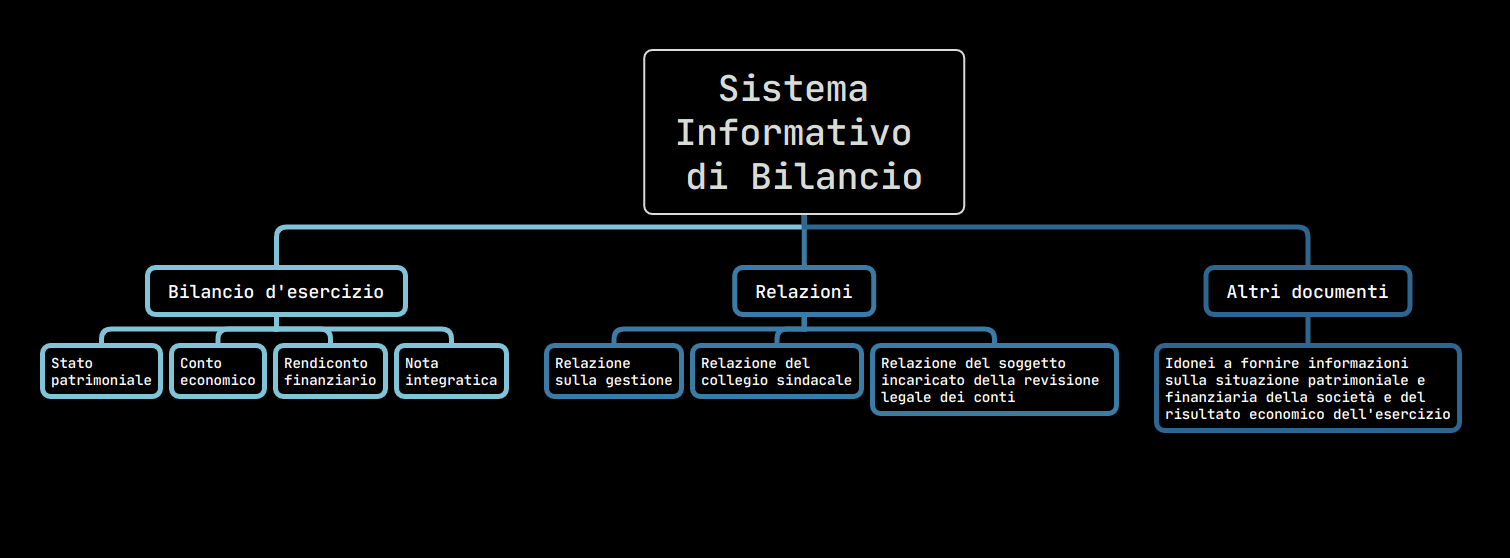
\includegraphics[width=0.75\textwidth]{./graphs/SistemaInformativoDiBilancioSchema.png}
\\
\subsection{La normativa sul bilancio}
\\
La normativa italiana sul bilancio d'esercizio, derivante dalla direttiva comunitaria 2013/34/UE, è integrata nel codice civile seguendo una struttura "dal generale al particolare". La clausola generale (art. 2423 c.c.) sottolinea la chiarezza e la rappresentazione veritiera della situazione patrimoniale e finanziaria. I principi di redazione e la struttura di Stato patrimoniale e Conto economico (artt. 2423 bis e 2423 ter c.c.) sono definiti, insieme al contenuto di Stato patrimoniale, Conto economico, Rendiconto finanziario e Nota integrativa (artt. 2424, 2425, 2425 ter, 2427 e 2427 bis c.c.). La normativa incorpora anche i criteri di valutazione degli elementi del patrimonio (art. 2426 c.c.). Attualmente, esistono quattro tipologie di bilancio con obblighi informativi crescenti in base alle dimensioni aziendali, e in caso di necessità, il bilancio può essere integrato con informazioni complementari per garantire una rappresentazione accurata.
\\
\subsection{Le componenti del bilancio d'esercizio civilistico}
\\
Il bilancio d'esercizio civile, composto da Stato patrimoniale, Conto economico, Rendiconto finanziario e Nota integrativa, riflette la situazione finanziaria, i risultati gestionali e i flussi finanziari. Derivati dal sistema informativo contabile, sono redatti in euro senza decimali, con possibili troncamenti o evidenziazioni in Riserve da arrotondamento. La finalità principale è rappresentare chiaramente la situazione patrimoniale, finanziaria ed economica per investitori, finanziatori e creditori. Lo Stato patrimoniale classifica elementi tra Attivo e Passivo secondo destinazione economica e fonti di finanziamento. Il Conto economico, derivato dalla Situazione economica finale, evidenzia risultati intermedi come la differenza tra valore e costi della produzione. La Nota integrativa fornisce informazioni aggiuntive seguendo l'ordine delle voci. Il sistema informativo contabile garantisce il raccordo tra le rilevazioni e il bilancio, permettendo riclassificazioni e prospetti di collegamento, disponibili per verifiche e ispezioni.
\\
\\
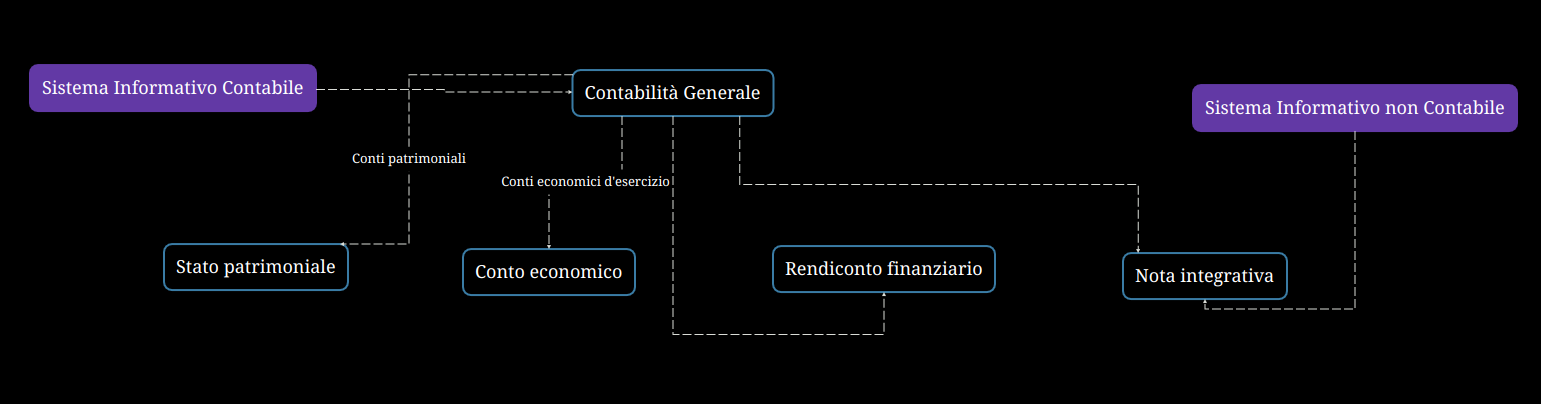
\includegraphics[width=0.75\textwidth]{./graphs/ComponentiDelBilanzioDesCivilisticoSchema.png}
\\
\\
\subsubsection{Schema di stato patrimoniale (Art. 2424 c.c.)}
\\
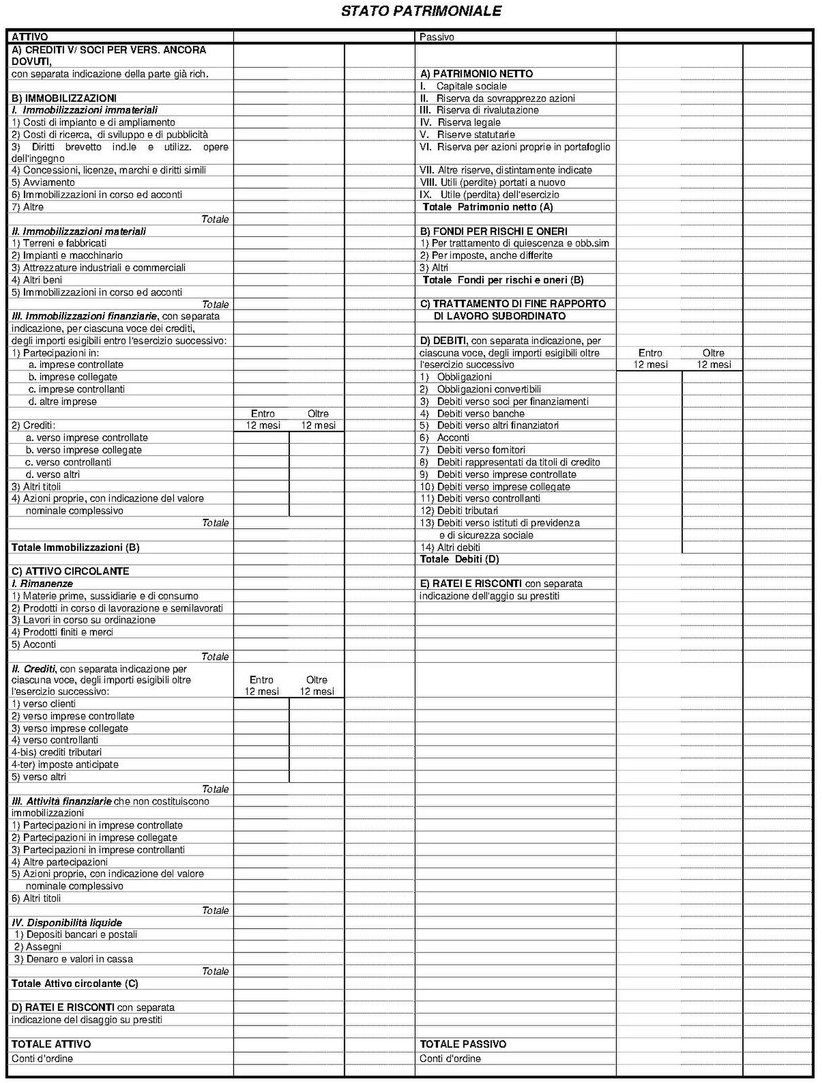
\includegraphics[width=0.75\textwidth]{./graphs/StatoPatrimoniale.png}
\\
\subsubsection{Schema di conto economico (Art. 2425 c.c.)}
\\
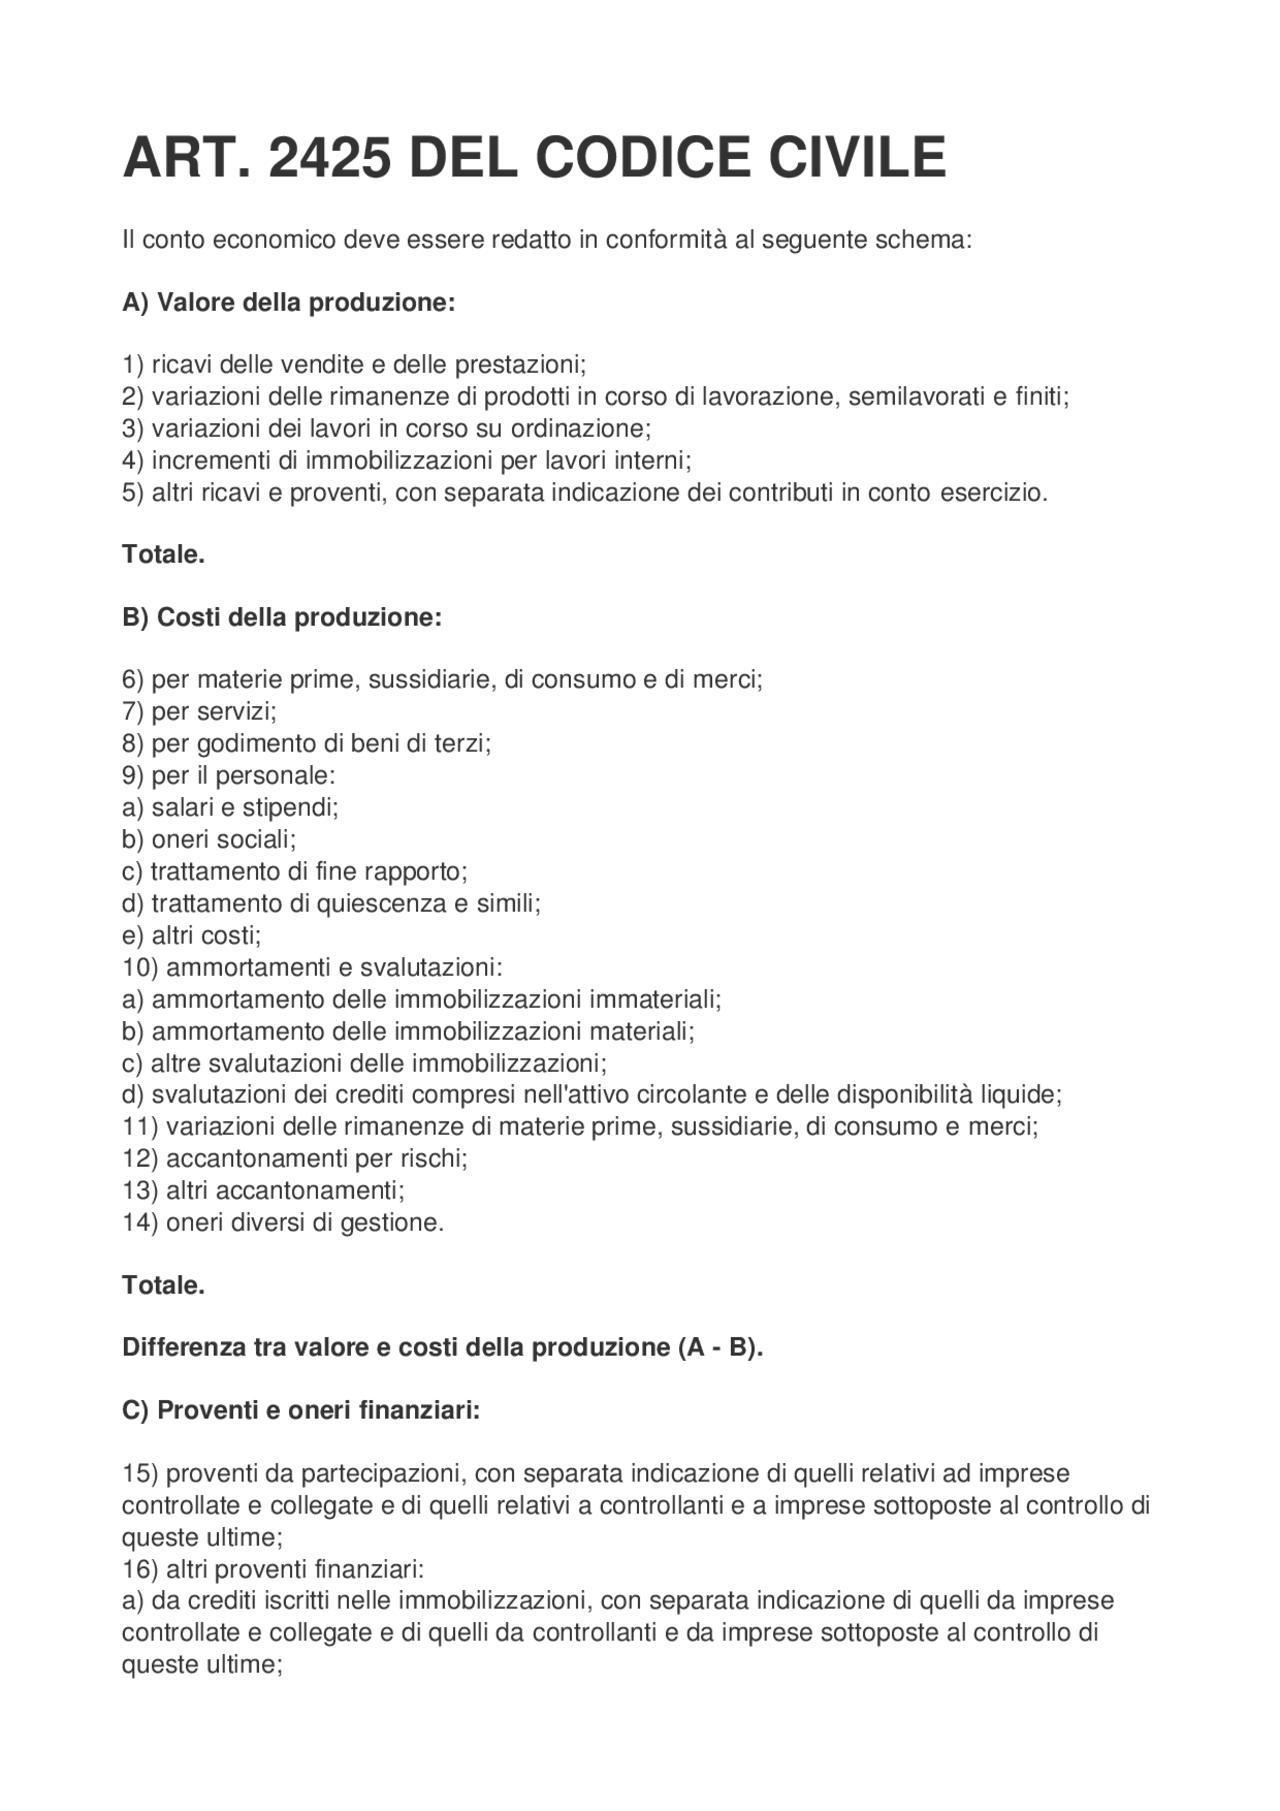
\includegraphics[width=0.75\textwidth]{./graphs/ContoEconomico.png}
\\
\subsection{Il bilancio in forma abbreviata e delle micro-imprese}
\\
Le società possono redigere il bilancio in forma abbreviata se, nel primo esercizio o successivamente per due esercizi consecutivi, non raggiungono due dei limiti stabiliti dall'art. 2435 bis del c.c.: un totale dell'attivo dello Stato patrimoniale di 4,400,000 euro, ricavi di vendite e prestazioni di 8,800,000 euro, e 50 dipendenti in media durante l'esercizio. Queste società sono esentate dal Rendiconto finanziario e hanno semplificazioni nello Stato patrimoniale, Conto economico e Nota integrativa. Le micro-imprese, che non superano i limiti dell'art. 2435 ter del c.c. (175,000 euro di totale attivo, 350,000 euro di ricavi, e 5 dipendenti in media), sono esentate dal Rendiconto finanziario e dalla Nota integrativa se forniscono le informazioni necessarie nel Calce dello Stato patrimoniale. Lo Stato patrimoniale e il Conto economico in forma abbreviata seguono la stessa struttura delle società in forma ordinaria. Gli amministratori delle società in forma abbreviata sono esonerati dalla redazione della relazione sulla gestione, a condizione che le informazioni richieste siano incluse nella Nota integrativa
\\
\subsection{I criteri di valutazione}
\\
I criteri di valutazione del patrimonio aziendale variano a seconda delle circostanze, come la situazione di funzionamento ordinario o scenari straordinari come cessione, liquidazione o fusione. Nell'impresa in funzionamento, la valutazione è complessa, poiché i beni sono interconnessi nel processo produttivo. Per evitare manipolazioni, si impongono vincoli giuridici (regole del codice civile) e vincoli tecnici (principi contabili). Questi vincoli mirano a garantire la coerenza nel tempo e nello spazio, evitando variazioni arbitrarie nei bilanci. Il codice civile specifica criteri di valutazione per diversi elementi patrimoniali, basati principalmente sul costo. Il principio della prudenza stabilisce il costo come massima valutazione, con alcune eccezioni, come lavori in corso su ordinazione. Le partecipazioni in imprese collegate possono essere valutate in base alla frazione del patrimonio netto. Gli strumenti finanziari derivati sono valutati al fair value, con variazioni contabilizzate nel Conto economico. È importante rispettare gli obblighi contabili, ma quando non influenzano la rappresentazione accurata, possono essere trascurati.
\\
\subsection{I principi contabili nazionali}
\\
I criteri di valutazione del codice civile, derivati dai principi di redazione del bilancio, sono fondamentali per rappresentare correttamente la situazione finanziaria dell'azienda. L'OIC, interpreta e rende operativi tali criteri tramite principi contabili. Questi si suddividono in principi contabili generali, che seguono l'art. 2423 bis e garantiscono una chiara rappresentazione del bilancio senza favoritismi, e principi contabili applicati, che dettano le regole specifiche per la composizione e l'esposizione delle voci nei bilanci. La neutralità del redattore è cruciale per l'attendibilità dei documenti contabili.
\\
\\
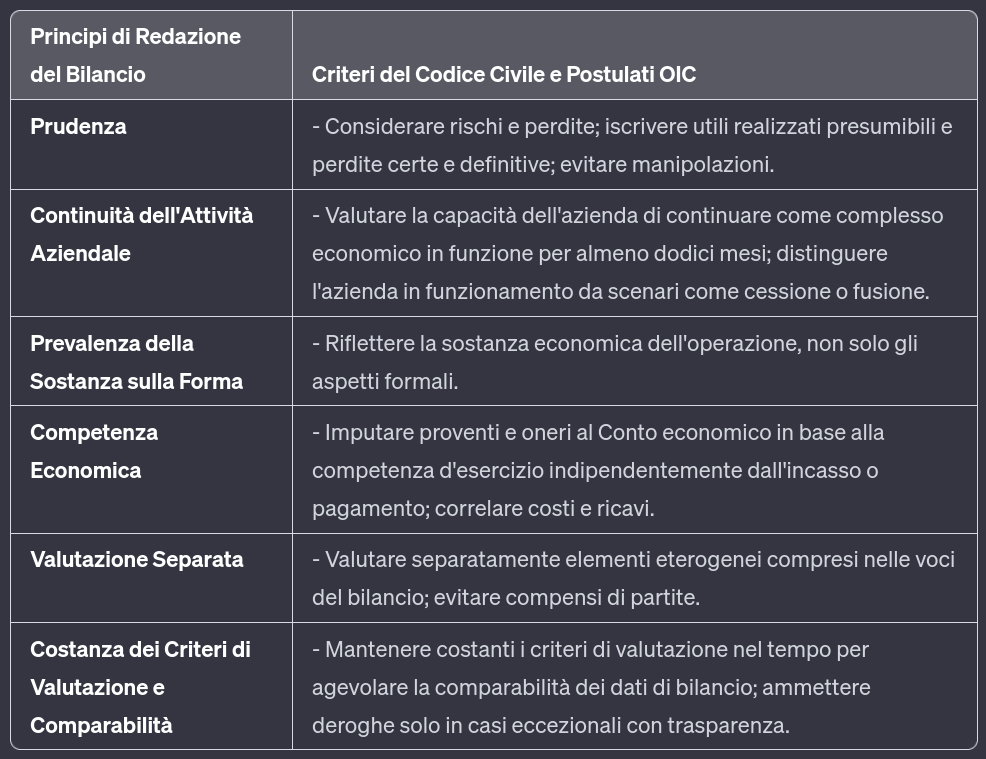
\includegraphics[width=0.75\textwidth]{./graphs/principiContabiliNazionali.png}
\\
\subsection{I principi contabili internazionali}
\\
La normativa vigente distingue tra società obbligate all'applicazione dei principi contabili internazionali (IAS/IFRS) e società con la facoltà di scegliere tra principi contabili internazionali e principi contabili nazionali. L'ambito di applicazione di tali principi varia a seconda della natura e delle caratteristiche delle società coinvolte
\\
\\
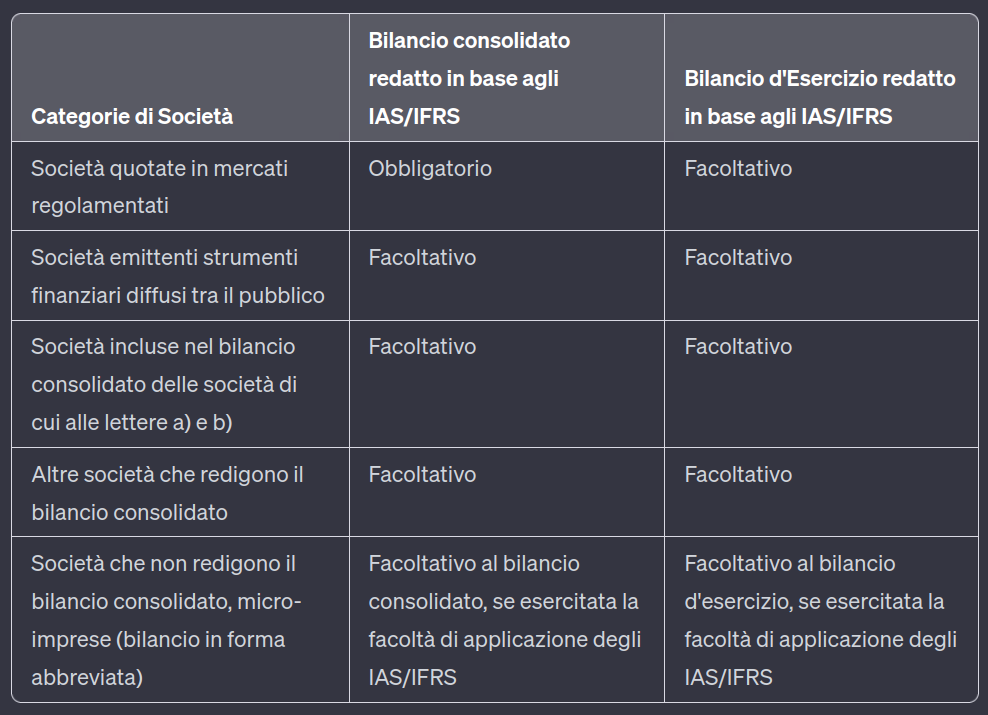
\includegraphics[width=0.75\textwidth]{./graphs/ambitoApplicazionePrincipiContabiliInternazionali.png}
\\
\\
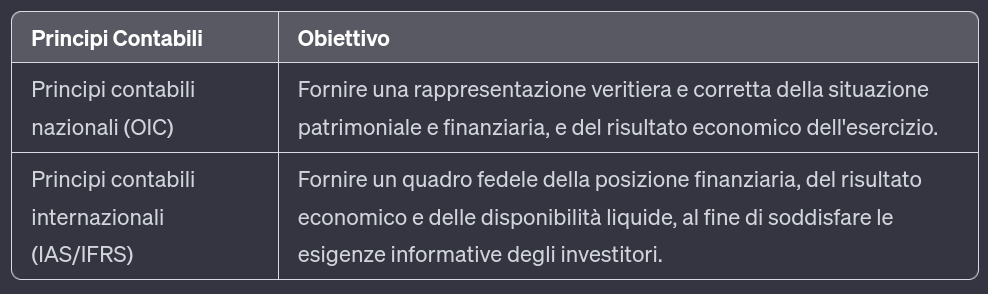
\includegraphics[width=0.75\textwidth]{./graphs/finalitàDelBilancioDesercizio.png}
\\
\\
Entrambi i principi, pur mantenendo sostanziali similitudini, presentano differenze significative, come l'approccio al fair value degli IAS/IFRS, che può influenzare l'attendibilità dei valori in bilancio ma accresce l'utilità per gli investitori
\\
\subsection{Il bilancio IAS/IFRS}
\\
Il bilancio d'esercizio redatto secondo i principi contabili internazionali comprende diversi documenti. Questi includono il Prospetto della situazione patrimoniale-finanziaria, il Prospetto di conto economico complessivo, il Prospetto delle variazioni di patrimonio netto e il Rendiconto finanziario, che fornisce informazioni sui flussi monetari durante l'esercizio. Le Note, simili alla Nota integrativa nazionale, integrano le informazioni fornite dai prospetti contabili.
\\
\\
I nomi dei prospetti non sono vincolanti, e le aziende possono scegliere denominazioni diverse, ma devono rispettare il contenuto minimo indicato. Nel Prospetto della situazione patrimoniale-finanziaria, le attività e passività sono distinte in correnti e non correnti, evidenziando gli importi scadenti o esigibili entro dodici mesi.
\\
\\
Il fair value è utilizzato per la valutazione di alcune voci, come le attività destinate alla dismissione. Le aziende possono scegliere di presentare il Prospetto di conto economico complessivo con due prospetti separati o un unico prospetto. Le Note al bilancio forniscono dettagli sugli schemi utilizzati, criteri di valutazione, informazioni supplementari per ciascuna voce e dettagli di settore. Gli IAS/IFRS richiedono anche una relazione degli organi amministrativi che descrive gli aspetti principali che influiscono sul risultato economico e sulla situazione finanziaria dell'impresa.
\\
\subsection{La relazione sulla gestione}
\\
La relazione sulla gestione, accompagnando il bilancio, è un documento essenziale per valutare la performance aziendale, andando oltre i dati contabili. Questo rapporto fornisce informazioni descriptive sui fatti principali dell'esercizio, integrate da dati quantitativi su settori specifici, come la redditività per segmenti specifici. Il suo obiettivo è consentire ai lettori del bilancio di comprendere l'andamento finanziario, inclusi piani d'investimento. Il codice civile stabilisce il contenuto minimo della relazione, richiedendo un'analisi completa della situazione aziendale, con particolare attenzione ai costi, ricavi, investimenti, rischi, e interazioni con l'ambiente e il personale. La relazione deve includere anche dettagli su ricerca e sviluppo, rapporti con altre imprese, azioni proprie, prospettive future e gestione dei rischi finanziari. La trasparenza è fondamentale, e la relazione deve riflettere le sedi secondarie dell'azienda.
\\
\subsection{La revisione legale}
\\
I conti annuali delle società di capitali, come il bilancio d'esercizio e, se redatto, il bilancio consolidato, sono sottoposti al controllo legale attraverso la procedura di revisione legale. Questa procedura, condotta da revisori legali o società di revisione legale iscritti nel Registro del Ministero dell'Economia e delle Finanze (MEF), verifica la correttezza della rappresentazione economica, finanziaria e patrimoniale dell'impresa nei bilanci.
\\
\\
Il soggetto incaricato della revisione varia a seconda del tipo di società. Società per azioni non quotate e non obbligate alla redazione del bilancio consolidato sono soggette al controllo legale in base all'art. 2409 bis del codice civile. Per le società quotate, enti di interesse pubblico, banche, e imprese di assicurazione, la revisione è disciplinata in modo più dettagliato.
\\
\\
L'organo incaricato della revisione legale, che può essere un revisore o una società di revisione, viene nominato nell'atto costitutivo o dall'assemblea dei soci. Questo incarico dura tre esercizi. La relazione di revisione attesta l'idoneità del bilancio a riflettere fedelmente la situazione aziendale. Il revisore deve essere indipendente dalla società e non può avere conflitti di interesse.
\\
\\
Il revisore deve effettuare controlli di qualità almeno ogni sei anni, verificando risorse, documenti di revisione, conformità ai principi di revisione, indipendenza e congruità dei compensi. Questi controlli sono eseguiti dalla CONSOB per i revisori all'interno di società di revisione e dal Ministero dell'Economia e delle Finanze per i revisori senza incarichi su enti di interesse pubblico.
\\
\subsection{Le attività di revisione contabile}
\\
I principi di revisione, noti come ISA (International Standard Auditing), hanno come obiettivo principale accrescere la fiducia degli utilizzatori del bilancio attraverso la formulazione di un giudizio sulla conformità del bilancio alle norme vigenti. La revisione contabile mira a ottenere elementi di prova sufficienti per attestare con ragionevole certezza l'affidabilità del bilancio, garantendo una rappresentazione veritiera della situazione patrimoniale, finanziaria ed economica dell'azienda.
\\
\\
Il processo di revisione è complesso e continuo, articolato attraverso diverse fasi interconnesse. La fase iniziale è la pianificazione, che consiste nella definizione di un piano di lavoro e nella programmazione delle attività. Questa fase è cruciale per limitare il rischio di formulare giudizi impropri sul bilancio, noto come rischio di revisione, derivante da inesattezze o anomalie non individuate durante i controlli.
\\
\\
Nella pianificazione, si identifica l'ambiente di controllo, che comprende il sistema informativo nella sua interezza, e si programmano le procedure e le aree aziendali soggette a revisione. La documentazione adatta a testimoniare la conformità ai principi di revisione è preparata in questa fase.
\\
\\
La documentazione del lavoro svolto dai revisori, chiamata carte di lavoro, deve essere conservata per dieci anni e resa disponibile durante i controlli periodici di qualità. Durante la revisione, il revisore deve applicare lo "scetticismo professionale", riconoscendo circostanze che potrebbero indicare errori significativi nel bilancio, come elementi di prova incoerenti, segnali di possibile frode e affidabilità dei documenti e delle risposte alle indagini.
\\
\\
Lo "scetticismo professionale" è particolarmente rilevante nelle revisioni delle stime aziendali, come il fair value, la riduzione del valore delle attività, gli accantonamenti, i flussi di cassa futuri e la continuità operativa dell'impresa.
\\
\\
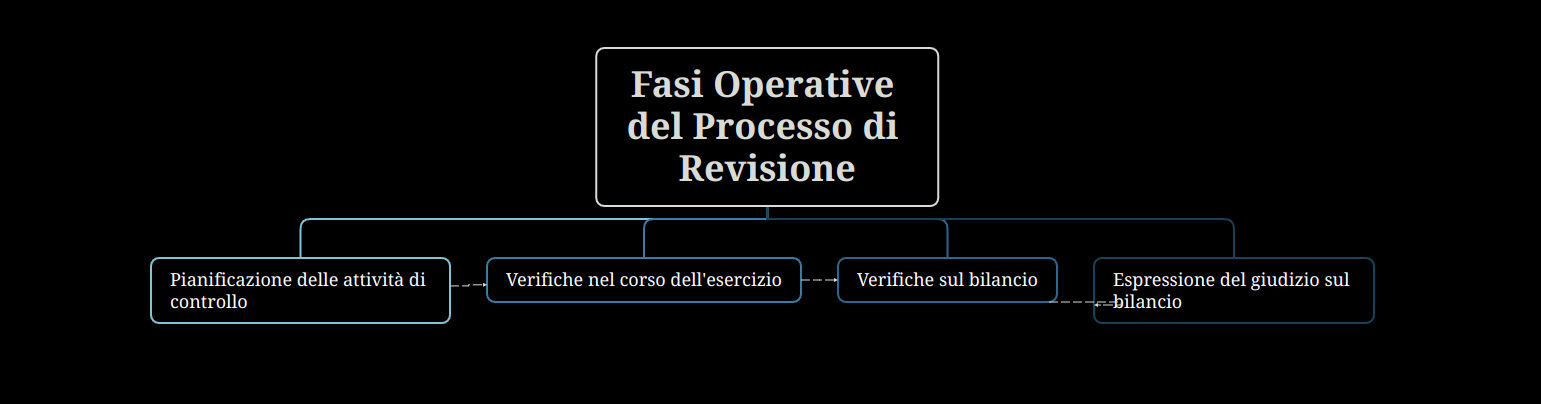
\includegraphics[width=0.75\textwidth]{./graphs/fasiOperativeDelProcessoDiRevisione.png}
\\
\subsection{Le verifiche nel corso dell'esercizio e sul bilancio}
\\
Il revisore legale analizza e formula un giudizio sulla conformità del bilancio alle norme contabili. Questo processo, continuo e complesso, coinvolge la pianificazione delle attività di controllo, la verifica nel corso dell'esercizio e le verifiche periodiche. Durante l'esercizio, il revisore controlla la regolare tenuta della contabilità, includendo la verifica degli obblighi legali legati ai libri e registri, nonché la corretta rilevazione delle operazioni di gestione. Le verifiche periodiche coinvolgono sondaggi su operazioni campione e un controllo più approfondito degli aggregati di bilancio significativi, garantendo la corretta aggregazione e classificazione delle voci e l'accuratezza delle informazioni riportate nella Nota Integrativa e nella Relazione sulla gestione.
\\
\subsection{La relazione e il giudizio sul bilancio}
\\
Al termine del processo di revisione, il revisore legale o la società di revisione legale emettono una relazione con un giudizio sul bilancio dell'esercizio. Il giudizio può essere positivo, senza modifica, o con modifica a seconda della conformità del bilancio alle norme. In caso di modifiche, vengono specificate le motivazioni. Il revisore esprime anche giudizi sulla coerenza della relazione sulla gestione con i dati del bilancio e sulla conformità della relazione alle norme di legge. La relazione segue una struttura predefinita che include sezioni introduttive, responsabilità del revisore, giudizio professionale sul bilancio e richiami di informativa, con eventuali aggiunte in caso di giudizio con modifica.
\\
\subsection{Esercizi Riepilogativi}
\\
\qs{Da cosa è costituito il sistema informativo di bilancio?}{Dall'insieme dei documenti costituiti dal bilancio d'esercizio (Stato Patrimoniale, Conto Economico, Rendiconto Finanziario e Nota Integrativa), dagli allegati, dalle informazioni complementari e dalle relazioni accompagnatorie (Relazione sulla gestione, Relazione del collegio sindacale, Relazione del soggetto incaricato alla revisione) e altri documenti idonei a fornire informazioni sulla situazione patrimoniale e finanziaria della società e del risultato economico dell esercizio}
\\
\\
\qs{Quale è la definizione di bilancio?}{Il bilancio d'esercizio è il documento redatto dagli organi amministrativi al termine del periodo amministrativo, con cui si rappresentano la situazione patrimoniale e finanziaria dell'azienda e il risultato economico dell'esercizio}
\\
\qs{Quali tipologie di bilancio prevede il codice civile?}{
  Il codice civile distingue 4 tipologie di biliancio con obblighi informativi crescenti a seconda delle dimensioni dell'azienda, queste tipologie sono:
  \begin{itemize}
    \item Il bilancio delle micro-imprese: E' redatto appunto dalle micro-imprese, entità che non superano i parametri stabiliti dall'articolo 2435 ter c.c.
    \item Il bilancio in forma abbreviata, E' redatto dalle società di minori dimensioni, imprese che non superano i parametri stabiliti dall'articolo 2435 bis c.c. 
    \item Il bilancio in forma ordinaria: E' redatto dalle società non quotate in mercati regolamentati e non emittenti azioni diffuse presso il pubblico in misura rilevante e che superano i parametri per la redazione del bilancio in forma abbreviata.
    \item Bilancio IAS/IFRS: E' redatto dalle società quotate in mercati regolamentati. Le società non quotate, pur se emittenti azioni diffuse presso il pubblico in misura rilevante, possono redigere il bilancio IAS/IFRS o, alternativamente il bilancio civilistico
  \end{itemize}
}
\\
\qs{Spiega quali sono i principi e le norme previste dalla normativa del bilancio?}{I principi e le norme previste dalla normativa del bilancio possono variare a seconda della legislazione vigente nel paese di riferimento. Tuttavia, in generale, ci sono alcuni concetti chiave e principi universali che spesso sono inclusi nelle normative contabili. Questi possono includere:
\begin{itemize}
  \item{Prudenza: L'adozione di valutazioni conservative nell'assegnare valori agli elementi patrimoniali e di conto economico.}
  \item{Corrispondenza: Collegare le entrate e le spese all'esercizio a cui si riferiscono, seguendo il principio di competenza.}
  \item{Continuità aziendale: Presupporre che l'azienda continuerà la sua attività in futuro, a meno che ci siano evidenze contrarie.}
  \item{Integrità e completezza delle informazioni: Fornire informazioni accurate e complete per consentire agli utenti di comprendere appieno la situazione finanziaria e operativa dell'azienda.}
  \item{Equità: Trattare tutte le parti interessate in modo giusto ed equo nei confronti delle informazioni contabili.}
\end{itemize}
Le norme possono anche includere requisiti specifici per la presentazione delle informazioni, l'elaborazione dei documenti contabili, la valutazione di determinati elementi e altro ancora. La normativa può variare notevolmente tra i diversi paesi e le diverse giurisdizioni.
}
\\
\newpage
\qs{Quale è la differenza tra bilancio consolidato e bilancio d'esercizio?}{Il bilancio d'esercizio e il bilancio consolidato sono due documenti contabili distinti che forniscono informazioni finanziarie su una società o un gruppo di società. Ecco le principali differenze tra i due:
\begin{itemize}
  \item{Ambito di applicazione:
    \begin{itemize}
      \item{Bilancio d'esercizio: Riguarda una singola società e presenta la situazione finanziaria, economica e patrimoniale di quell'azienda specifica durante un periodo contabile, solitamente di 12 mesi.}
      \item{Bilancio consolidato: Incorpora i dati finanziari di tutte le società controllate dal gruppo, mostrando la situazione finanziaria complessiva del gruppo.}
    \end{itemize}
  }
  \item{Contenuto:
    \begin{itemize}
      \item{Bilancio d'esercizio: Contiene informazioni specifiche e dettagliate sulla singola società, inclusi asset, passività, redditi e spese.}
      \item{Bilancio consolidato: Incorpora i dati finanziari di tutte le società controllate dal gruppo, mostrando la situazione finanziaria complessiva del gruppo.}
    \end{itemize}
  }
  \item{Obiettivi:
    \begin{itemize}
      \item{Bilancio d'esercizio: Serve a valutare la performance finanziaria di una singola entità e a fornire informazioni per decisioni interne ed esterne.}
      \item{Bilancio consolidato: Fornisce una visione più ampia della salute finanziaria di un intero gruppo di società, importante per gli investitori e altri stakeholder interessati alla performance del gruppo nel suo insieme.}
    \end{itemize}
  }
  \item{Processo di Consolidamento:
    \begin{itemize}
      \item{Bilancio d'esercizio: Non coinvolge il processo di consolidamento, poiché rappresenta solo i dati di un'entità aziendale specifica.}
      \item{Bilancio consolidato: Richiede il consolidamento dei dati finanziari delle diverse società del gruppo, considerando e eliminando eventuali transazioni interne tra di esse per evitare la duplicazione dei dati.}
    \end{itemize}
  }
\end{itemize}
}
\\
\qs{Che cosa è il bilancio civilistico e come è composto il bilancio civilistico?}{Il bilancio civilistico è un documento contabile che le aziende redigono in conformità alle norme civilistiche. È uno strumento fondamentale per rappresentare la situazione economica, finanziaria e patrimoniale dell'azienda in un dato periodo. Il bilancio civilistico è spesso richiesto dalla normativa vigente per le società di capitali (come le società per azioni o le società a responsabilità limitata) e deve essere preparato secondo le disposizioni del Codice Civile italiano.}
\\
\qs{Quale è la differenza tra bilancio in forma ordinaria e bilancio civilistico?}{Il termine "bilancio in forma ordinaria" non è un'espressione standardizzata nel contesto contabile o legale. Di solito, si fa riferimento al "bilancio ordinario" o al "bilancio d'esercizio" per indicare il documento contabile annuale preparato da un'azienda secondo le normative di bilancio vigenti.
\\
\\
D'altra parte, il "bilancio civilistico" è un termine più specifico e si riferisce al bilancio preparato in conformità alle norme civilistiche, principalmente definite dal Codice Civile italiano. Quindi, la domanda potrebbe essere formulata in modo errato o potrebbe esserci un malinteso tra "bilancio in forma ordinaria" e "bilancio civilistico".}
\\
\qs{Cosa si intende con riserva di arrotondamento nel bilancio civilistico}{Il bilancio civilistico è redatto in euro senza decimali, ciò comporta una problematica a livello di arrotondamenti, in tal caso il bilancio rimane troncato senza pareggio contabile oppure la differenza viene evidenziata, rispettivamente in un'apposita riserva da arrotondamento (Voce altre riserve tra le parti ideali del patrimonio netto) nello Stato patrimoniale o nel conto economico a seconda che sia positivo o negativo}
\\
\qs{Elenca i criteri per eseguire il bilancio in forma abbreviata o delle micro-imprese?}{
  In base alla normativa italiana, le micro-imprese e le piccole imprese possono beneficiare della possibilità di redigere il bilancio in forma abbreviata. Tuttavia, i criteri per avvalersi di questa semplificazione possono variare a seconda del tipo di impresa. Di seguito sono elencati i principali criteri per eseguire il bilancio in forma abbreviata per le micro-imprese:
  \begin{itemize}
    \item{Criteri per le Micro-imprese:
          \begin{itemize}
            \item{Ammontare dell'Attivo Totale: Le micro-imprese sono generalmente caratterizzate da un ammontare dell'attivo totale non superiore a 175.000 euro.}
            \item{Ricavi delle Vendite e delle Prestazioni: I ricavi delle vendite e delle prestazioni non devono superare i 350.000 euro.}
            \item{Numero Medio dei Dipendenti: Il numero medio dei dipendenti durante l'esercizio non deve superare i 5 unità.}
          \end{itemize}
    }
  \item{Criteri per eseguire il bilancio in forma abbreviata:
       \begin{itemize}
        \item{Ammontare dell'Attivo Totale: Le piccole imprese possono usufruire della forma abbreviata se l'ammontare dell'attivo totale è inferiore a 4 milioni e 4 cento mila euro.}
        \item{Ricavi delle Vendite e delle Prestazioni: I ricavi delle vendite e delle prestazioni non devono superare i 8 milioni e 8 cento mila euro.}
        \item{Numero Medio dei Dipendenti: Il numero medio dei dipendenti durante l'esercizio non deve superare i 50.}
       \end{itemize}
    }
  \end{itemize}
}
\\
\qs{Quali sono le agevolazioni previste per il bilancio in forma abbreviata e micro-imprese?}{L'adozione del bilancio in forma abbreviata comporta alcune agevolazioni e semplificazioni, soprattutto in termini di allegati e dettagli da presentare nel documento contabile. Ecco alcune delle principali agevolazioni previste per il bilancio in forma abbreviata:
\begin{itemize}
  \item{Alleggerimento delle Informazioni da Presentare: La forma abbreviata richiede la presentazione di un numero ridotto di informazioni rispetto a un bilancio redatto in forma ordinaria o civilistica.}
  \item{Semplificazione della Relazione sulla Gestione: La relazione sulla gestione, se richiesta, può essere redatta in forma sintetica rispetto a quella prevista per un bilancio ordinario.}
  \item{Esenzione da Alcuni Documenti: L'impresa che adotta la forma abbreviata è esonerata dalla presentazione di alcuni documenti, contribuendo a semplificare la documentazione contabile complessiva.}
  \item{Minore Dettaglio nelle Note Integrative: Le note integrative, che forniscono dettagli e spiegazioni sulle voci del bilancio, possono essere redatte in forma più sintetica rispetto ai requisiti previsti per la forma ordinaria.}
  \item{Maggiore Agilità nell'Adempimento degli Obblighi Contabili: L'adozione della forma abbreviata è finalizzata a offrire alle imprese una maggiore agilità nell'adempimento degli obblighi contabili, riducendo la complessità delle procedure.}
  \item{Riduzione dei Costi di Redazione: La semplificazione delle procedure e la riduzione del dettaglio richiesto contribuiscono a contenere i costi di redazione del bilancio.}
\end{itemize}}
\\
\qs{Che cosa sono e a che cosa servono i criteri di valutazione previsti dalla normativa attuale?}{ criteri di valutazione rappresentano linee guida e regole stabilite dalla normativa contabile per determinare come gli elementi patrimoniali e finanziari devono essere valutati e rappresentati nel bilancio. 
\\
\\
Servono a garantire che il bilancio offra una rappresentazione fedele e accurata della situazione economica, finanziaria e patrimoniale dell'azienda, consentendo agli utenti di comprendere la sua posizione e prestazione.}
\\
\qs{Che cosa si intende con costo storico e costo ammortizzato?}{Il costo storico e il costo ammortizzato sono due differenti approcci utilizzati per la valutazione e la registrazione di determinati elementi patrimoniali nelle pratiche contabili. Ecco una spiegazione di entrambi i concetti:
\begin{itemize}
  \item{Costo Storico: Il costo storico è un principio contabile che prevede che gli elementi del bilancio siano registrati in base al valore iniziale o al costo effettivo sostenuto dall'azienda al momento dell'acquisizione. In altre parole, gli asset sono registrati nel bilancio al costo pagato o al valore di
mercato al momento dell'acquisizione.
    \\
    \\
Questo approccio è particolarmente applicato a beni tangibili come terreni, fabbricati e macchinari. Ad esempio, se un'azienda acquista un immobile per 100.000 euro, il costo storico di tale attivo sarà registrato nel bilancio a 100.000 euro, indipendentemente dal suo valore di mercato attuale.}
  \item{Costo Ammortizzato:

    Il costo ammortizzato è un approccio utilizzato principalmente per la valutazione di strumenti finanziari come prestiti o obbligazioni. In questo caso, il costo ammortizzato tiene conto non solo del valore nominale dell'investimento, ma anche degli interessi accumulati e degli eventuali sconti o premi.
    \\
    \\
L'ammortamento del costo riflette il riconoscimento graduale delle componenti finanziarie nel tempo. Ad esempio, se un'azienda detiene un prestito con un tasso di interesse, il costo ammortizzato terrà conto degli interessi maturati in modo che il valore contabile rifletta il costo effettivo dell'investimento al momento di qualsiasi registrazione contabile.}
\end{itemize} }
\\
\qs{Spiega che cosa si intende e come è composto con il termine bilancio ias/ifrs}{Il termine "IAS/IFRS" si riferisce agli standard internazionali di contabilità (IAS) e agli International Financial Reporting Standards (IFRS). Questi standard sono sviluppati e gestiti dall'International Accounting Standards Board (IASB). Il bilancio redatto secondo gli IAS/IFRS è progettato per essere utilizzato a livello internazionale, garantendo una maggiore uniformità e comparabilità delle informazioni finanziarie tra le diverse aziende.}
\\
\qs{Che cosa è e come viene effettuata la relazione sulla gestione}{La relazione sulla gestione è un documento aziendale che accompagna i rendiconti finanziari, fornendo ulteriori informazioni sulle attività, sulla situazione finanziaria e sui risultati della società. Essa offre una visione più approfondita delle attività e delle strategie adottate dalla direzione nell'arco dell'esercizio finanziario. La relazione sulla gestione viene anch'essa redatta dagli amministratori da tale relazione devono emergere: 
\begin{itemize}
  \item Le attività di ricerca e sviluppo
  \item I rapporti con imprese controllate controllanti collegate
  \item Il numero e il valore delle azioni proprie e quote di società possedute
  \item L'evoluzione prevedibile della gestione
\end{itemize}
}
\\
\qs{Revisione legale}{La revisione legale è un insieme di attività (monitoraggi e verifiche) con cui si sottopongono al controllo legale il bilancio d'esercizio e, se redatto, il bilancio consolidato. Al termine di tale procedura il soggetto incaricato del controllo deve esprimere un giudizio sul bilancio, attestando con una specifica relazione l'idoneità del bilancio stesso arappresentare correttamente e in modo veritiero la reale situazione economica finanziaria e patrimoniale dell'impresa}
\\
\\
\qs{Spiega come vengono effettuate e da chi le verifiche nel corso del esercizio e sul bilancio}{Le verifiche nel corso dell'esercizio sono un aspetto cruciale del processo di revisione contabile e coinvolgono diversi aspetti dell'attività aziendale per garantire la correttezza delle informazioni finanziarie. Queste verifiche sono eseguite da revisori legali o società di revisione legali e seguono un approccio sistematico 
\begin{itemize}
  \item{Verifiche nel Corso dell'Esercizio:
\\
\\
Regolare Tenuta della Contabilità: Una delle verifiche principali è quella sulla regolare tenuta della contabilità. Si controlla che l'azienda adempia a tutti gli obblighi di legge relativi ai libri e ai registri contabili. Ciò include la verifica della correttezza formale, tempistica e accuratezza delle registrazioni.
\\
\\
Analisi dei Libri Contabili e Registri Obbligatori: Si effettua un attento esame dei libri contabili e dei registri obbligatori. Questo assicura la conformità alle norme di legge e l'adeguata registrazione delle operazioni aziendali.
\\
\\
Dichiarazioni e Versamenti Tributari: Si verificano le dichiarazioni, le liquidazioni periodiche e i versamenti tributari e previdenziali. Questa fase assicura che l'azienda rispetti tutti gli obblighi fiscali e previdenziali in termini di tempestività e accuratezza delle registrazioni.
\\
\\
Contenuto dei Verbali delle Riunioni degli Organi Collegiali: Si esamina il contenuto dei verbali delle riunioni degli organi collegiali, come il consiglio di amministrazione o il collegio sindacale. Questo è importante per comprendere le decisioni prese e le eventuali implicazioni finanziarie.}
\item{Verifiche sul Bilancio:
\\
\\
Analisi degli Aggregati di Bilancio: Dopo aver acquisito elementi di prova durante le verifiche nel corso dell'esercizio, si procede all'analisi degli aggregati di bilancio ritenuti più significativi. Ciò include elementi come immobilizzazioni immateriali, materiali, finanziarie, crediti, ecc.
\\
\\
Controllo dell'Aggregazione e Classificazione delle Voci: Il controllo si concentra sulla corretta aggregazione e classificazione delle voci nel bilancio. Si verifica che le informazioni siano presentate in modo accurato e conforme alle normative contabili.
\\
\\
Relazione sulla Gestione e Giudizio di Coerenza: Il revisore deve rilasciare un giudizio sulla relazione sulla gestione e verificare la sua coerenza con i dati del bilancio. Questo assicura una rappresentazione accurata e veritiera della situazione aziendale.}
\end{itemize}}
\\
\newpage
\qs{Spiega la relazione e il giudizio sul bilancio come e da chi viene eseguito}{La relazione e il giudizio sul bilancio rappresentano il culmine del processo di revisione contabile, e sono compiuti dal soggetto incaricato della revisione, che può essere un revisore legale o una società di revisione legale. Di seguito, vengono spiegate le fasi chiave di questo processo.
\\
\\
Formulazione del Giudizio:
Al termine del processo di revisione, il revisore legale o la società di revisione legale deve formulare un giudizio sul bilancio dell'esercizio e, se redatto, sul bilancio consolidato.
\\
\\
Struttura e Contenuto della Relazione:
La struttura e il contenuto della relazione, insieme alle tipologie di giudizio, sono regolamentati dal principio di revisione internazionale - ISA Italia 700. Questo assicura coerenza e uniformità nelle relazioni di revisione.
\\
\\
Tipologie di Giudizio:
Il revisore può esprimere diverse tipologie di giudizio:
\\
a) Giudizio Senza Modifica (Positivo): Si formula quando si ritiene di aver acquisito elementi probativi sufficienti e appropriati, attestando la conformità del bilancio alle normative sull'informazione finanziaria.
\\
b) Giudizio con Modifica: Questo può includere varie categorie, come giudizio con rilievi, giudizio negativo o dichiarazione di impossibilità di esprimere un giudizio. La scelta dipende dalla significatività e pervasività degli errori riscontrati.
\\
\\
Analisi Dettagliata in Caso di Modifica:
Nel caso di un giudizio con modifica, il revisore deve indicare analiticamente le motivazioni alla base della decisione nella relazione al bilancio. Questo fornisce una spiegazione dettagliata degli elementi che hanno influenzato il giudizio.
\\
\\
Giudizio sulla Coerenza della Relazione sulla Gestione:
Il revisore deve rilasciare un giudizio sulla coerenza della relazione sulla gestione con i dati del bilancio. Ciò assicura che le informazioni presentate nella relazione sulla gestione siano in linea con i risultati finanziari riflessi nel bilancio.
\\
\\
Richiami di Informativa:
Il revisore può includere richiami di informativa, evidenziando informazioni rilevanti che meritano particolare attenzione degli utilizzatori del bilancio.
\\
\\
Relazione Strutturata e Standardizzata:
La relazione sulla revisione segue una struttura predefinita, con sezioni introduttive e specifiche sulla responsabilità del revisore, giudizio professionale sul bilancio, richiami di informativa, e, in caso di modifica, una sezione dettagliata sugli elementi alla base del giudizio.}
\\
\qs{Che cosa è il rendiconto finanziario?}{fornisce un'istantanea della situazione finanziaria di un'azienda in un determinato momento. Esso presenta la posizione finanziaria netta dell'azienda, indicando la differenza tra le risorse finanziarie (attività) e le fonti di finanziamento (passività) al momento della redazione del rendiconto.}
% section Bilanci Aziendali e Revisione Legale dei Conti (end)

% chapter Contabilità Generale e Bilancio (end)

\chapter{Piano dei conti di una società per azioni (con attività industriale)} % (fold)
\label{chap:Piano dei conti}

\begin{multicols}{2}
\begin{description}
  \item[Crediti V/Soci]
    \begin{itemize}
      \item Azionisti c/sottoscrizione;
      \item Azionisti c/versamenti richiamati;
      \item Azionisti c/reintegro.
    \end{itemize}
    \nt{Il raggruppamento accoglie conti finanziari accesi ai crediti, generalmente a breve
termine. Il codice civile richiede la separata indicazione della parte già richiamata.}
  \item[Immobilizzazioni Immaterial]
    \begin{itemize}
      \item Costi di Impianto;
      \item Costi di Ampliamento;
      \item Costi di Sviluppo;
      \item Brevetti industriali;
      \item Software;
      \item Concessioni e licenze;
      \item Avviamento;
      \item Fondo ammort. costi di Impianto;
      \item Fondo ammort. costi di Ampliamento;
      \item Fondo ammort. costi di Sviluppo;
      \item Fondo ammort. Brevetti industriali;
      \item Fondo ammort. Software;
      \item Fondo ammort. Concessioni di licenze;
      \item Fondo ammort. Avviamento;
      \item Fondo svalutazione Brevetti industriali;
      \item Immobilizzazioni immateriali in corso;
      \item Fornitori Immobilizzazioni immateriali c/acconti.
    \end{itemize}
    \nt{I costi relativi all'installazione, all'ampliamento, alla ricerca, allo sviluppo e alla pubblicità possono essere registrati nel bilancio come immobilizzazioni con il consenso del collegio sindacale, se presente. Il costo del software di base viene contabilizzato insieme all'hardware.
\\
\\
Il costo del software applicativo viene registrato nella voce B I 3 se acquistato come proprietà o licenza d'uso a tempo indeterminato, o se prodotto in economia e tutelato dalla normativa sui diritti d'autore. Se acquistato come licenza d'uso a tempo determinato con pagamento di un corrispettivo una tantum, viene iscritto nella voce B I 4. Se prodotto in economia senza ottenere la tutela giuridica, viene registrato nella voce B I 7.
\\
\\
L'avviamento può essere incluso tra le immobilizzazioni entro i limiti del prezzo pagato a tale scopo, previo consenso del collegio sindacale, se presente. I fondi ammortamento sono utilizzati per ridurre il valore delle voci a cui si riferiscono nel bilancio.}

  \item[Immobilizzazioni Materiali]
    \begin{itemize}
      \item Terreni e Fabbricati;
      \item Impianti e macchinari;
      \item Attrezzature Industriali;
      \item Attrezzature Commerciali;
      \item Macchine d'ufficio;
      \item Arredamento;
      \item Automezzi;
      \item Imballaggi durevoli;
      \item Fondo ammort. Terreni e Fabbricati;
      \item Fondo ammort. Impianti e macchinari;
      \item Fondo ammort. Attrezzature industriali;
      \item Fondo ammort. Attrezzature Commerciali;
      \item Fondo ammort. Macchine d'ufficio;
      \item Fondo ammort. Arredamento;
      \item Fondo ammort. Automezzi;
      \item Fondo ammort. Imballaggi durevoli;
      \item Fondo svalutazione terreni e fabbricati;
      \item Fondo svalutazione impianti e macchinari;
      \item Immobilizzazioni in corso;
      \item Fornitori immobilitazioni materiali c/acconti.
    \end{itemize}
    \nt{I fondi ammortamento e i fondi svalutazione sono portati in diminuzione delle voci a cui si riferiscono.}
  \item[Immobilizzazioni Finanziarie]
    \begin{itemize}
      \item Partecipazioni in controllate;
      \item Partecipazioni in collegate;
      \item Partecipazioni in controllanti;
      \item Partecipazioni diverse;
      \item Prestiti a controllate;
      \item Prestiti a collegate;
      \item Prestiti a controllanti;
      \item Mutui attivi v/terzi; SP (Attivo) B III 2 d) Crediti verso altri
      \item Azioni proprie;
      \item Titoli immobilizzati. SP (Attivo) B III 3) altri titoli
    \end{itemize}
\nt{Il raggruppamento accoglie conti economici accesi ai costi sospesi (relativamente ai titoli di debito e di capitale detenuti per esigenze strategiche) e conti finanziari accesi ai crediti.Per ciascuna voce dei crediti deve essere indicato l’importo esigibile nell’esercizio successivo.}
  \item[Rimanenze]
    \begin{itemize}
      \item Materie prime;
      \item Materie sussidiarie;
      \item Materie di consumo;
      \item Prodotti in lavorazione;
      \item Semilavorati;
      \item Lavori in corso su ordinazione;
      \item Prodotti finiti;
      \item Fornitori materie c/acconti.
    \end{itemize}
  \nt{Il raggruppamento accoglie conti economici accesi ai costi sospesi, salvo il conto "Materie Prime" Fornitori materie c/acconti che è un conto finanziario acceso a crediti.}
  \item[Crediti Commerciali]
    \begin{itemize}
      \item Crediti v/clienti; (crediti verso clienti)
      \item Crediti Commerciali diversi; (crediti verso clienti)
      \item Clienti c/costi anticipati; (crediti verso clienti)
      \item Crediti fattorizzati; 
 (crediti verso clienti)
      \item Cambiali attive; (crediti verso clienti)
      \item Cambiali allo sconto; (crediti verso clienti)
      \item Cambiali all'incasso; (crediti verso clienti)
      \item Fatture da emettere; (crediti verso clienti)
      \item Crediti insoluti; (crediti verso clienti)
      \item Cambiali insolute; (crediti verso clienti)
      \item Crediti da liquidare; (crediti verso clienti)
      \item Crediti per acconti da clienti; (crediti verso clienti)
      \item Crediti v/controllate;
      \item Crediti v/collegate;
      \item Crediti v/controllanti;
      \item Fondo svalutazione crediti; (In retifica a crediti verso clienti)
      \item Fondo rischi su crediti. (In retifica a crediti verso clienti)
    \end{itemize}
  \nt{Per ciascuna voce dei crediti deve essere indicato l’importo esigibile oltre l’esercizio successivo. Il raggruppamento crediti commerciali accoglie conti finanziari accesi a crediti di regolamento e alle loro rettifiche; in particolare i conti Fondo svalutazione crediti e Fondo rischi su crediti rettificano il valore nominale dei crediti, in funzione del rischio specifico e del rischio globale di perdite nel realizzo dei crediti stessi.}
  \item[Crediti diversi]
    \begin{itemize}
      \item Iva ns/credito; (Non affluisce in bilancio in quanto il saldo è girato al conto IVA c/liquidazione)
      \item Imposte c/acconti; (Non affluisce in bilancio in quanto il saldo si compensa con il
        debito per le imposte di competenza dell’esercizio)
      \item Crediti per ritenute subite; (Non affluisce in bilancio in quanto il saldo si compensa con il
debito per le imposte di competenza dell’esercizio)
      \item Crediti d'imposta; (Non affluisce in bilancio in quanto il saldo si compensa con il
debito per le imposte di competenza dell’esercizio)
      \item Crediti per iva; (SP (Attivo) C II 4bis) crediti tributari)
      \item Iva c/acconto; (Non affluisce in bilancio in quanto il saldo è girato al conto IVA c/liquidazione)
      \item Attività per imposte anticipate; (SP (Attivo) C II 4bis) crediti tributari)
      \item Crediti per cauzioni; (SP (Attivo) C II 5) crediti verso altri)
      \item Personale c/acconti; (SP (Attivo) C II 5) crediti verso altri)
      \item Crediti v/istituti previdenziali; (SP (Attivo) C II 5) crediti verso altri)
      \item Crediti diversi; (SP (Attivo) C II 5) crediti verso altri)
      \item Obbligazionisti c/sottoscrizione; (SP (Attivo) C II 5) crediti verso altri)
      \item Ente concedente c/contributi. (SP (Attivo) C II 5) crediti verso altri)
    \end{itemize}
    \nt{Il raggruppamento crediti diversi accoglie conti finanziari accesi a crediti verso una pluralità di debitori diversi.}

  \item[Attività finanziarie]
    \begin{itemize}
      \item Partecipazioni; (SP (Attivo) C III 4) altre partecipazioni)
      \item Azioni proprie da annullare
      \item Titoli; (SP (Attivo) C III 6) altri titoli)
      \item Obbligazioni sociali; (SP (Attivo) C III 6) altri titoli)
    \end{itemize}
  \nt{Il raggruppamento accoglie conti economici accesi ai costi sospesi relativi a titoli di capitale e di debito destinati a permanere nel patrimonio aziendale per periodi brevi.}
  \item[Dispnibilità liquide]
    \begin{itemize}
      \item Banche c/c attivi;
      \item Banca c/vincolato;
      \item C/c postali;
      \item Assegni;
      \item Denaro in cassa;
      \item Valori bollati;
    \end{itemize}
    \nt{Il raggruppamento accoglie conti finanziari accesi ai crediti a vista e ai valori in cassa.}
  \item[Ratei e Risconti Attivi]
    \begin{itemize}
      \item Ratei attivi;
      \item Risconti attivi;
      \item Disaggio su prestiti.
    \end{itemize}
    \nt{Il disaggio su prestiti è una immobilizzazione immateriale, tuttavia il codice civile impone la sua iscrizione alla voce Ratei e risconti.}
  \item[Patrimonio Netto]
    \begin{itemize}
      \item Capitale sociale;
      \item Riserva Sovraprezzo azioni;
      \item Riserva di rivalutazione;
      \item Riserva legale;
      \item Riserva statutaria;
      \item Riserva conguaglio utili in corso;
      \item Fondo rimborso spese
      \item Versamenti azionisti c/capitale;
      \item Versamenti c/aumento capitale;
      \item Riserva rivalutazione partecipazioni;
      \item Riserva conversione obbligazioni;
      \item Utili a nuovo;
      \item Perdita d'esercizio;
      \item Riserva negativa per azioni proprie.
    \end{itemize}
    \nt{Il raggruppamento accoglie conti economici di patrimonio netto, accesi alle sue parti ideali, positive e negative.}
  \item[Fondi per rischi e oneri]
    \begin{itemize}
      \item Fondo per imposte;
      \item Fondo imposte differite;
      \item Fondo responsabilità civile;
      \item Fondo garanzie prodotti;
      \item Fondo manutenzioni programmate;
      \item Fondo operazioni e concorsi a premio.
    \end{itemize}
    \nt{Il Fondo per imposte comprende le passività per imposte probabili, il cui ammontare o la cui data di sopravvenienza siano indeterminati, quali accertamenti non definitivi e contenziosi in corso. Le sue contropartite sono: Oneri fiscali diversi se trattasi di imposte indirette imputabili all’esercizio; Imposte dell’esercizio, se trattasi di accantonamenti per imposte dirette imputabili all’esercizio; Imposte relative a esercizi precedenti se trattasi di accantonamenti imputabili a esercizi precedenti (oneri straordinari). Il Fondo imposte differite accoglie le imposte dirette che, pur essendo di competenza dell’esercizio, si renderanno esigibili solo in esercizi futuri (imposte differite).}
  \item[Trattamento fine rapporto]
    \begin{itemize}
      \item Debiti per TFR
    \end{itemize}
  \item[Debiti finanziari]
    \begin{itemize}
      \item Prestiti obbligazionari;
      \item Prestiti obbligazionari convertibili;
      \item Azionisti c/finanziamenti; (SP (Passivo) D 3) debiti verso soci per finanziamenti)
      \item Banche c/passivi;
      \item Banche c/Ri.Ba. sbf;
      \item Banche c/cambiali sbf;
      \item Banche c/anticipi su fatture;
      \item Banche c/sovvenzioni cambiarie;
      \item Banche c/sovvenzioni garantite;
      \item Banche c/interessi maturati;
      \item Mutui passivi;
      \item Prestiti da controllate;
      \item Prestiti da collegate;
      \item Prestiti da controllanti;
      \item Debiti v/altri finanziatori.
    \end{itemize}
    \nt{La voce D "Debiti" comprende tutte le passività per le quali sono certi e determinati sia l'importo che la data di scadenza. Per ogni specifica categoria di debiti, è necessario indicare l'importo dovuto oltre l'esercizio successivo. Il raggruppamento "Debiti finanziari" include i conti finanziari che costituiscono passività di finanziamento.}
  \item[Debiti Commerciali]
    \begin{itemize}
      \item Clienti c/acconti;
      \item Debiti v/fornitori;
      \item Debiti per acconti a fornitori;
      \item Fatture da ricevere;
      \item Cambiali passive. (SP (Passivo) D 8) debiti rappresentati da titoli di credito)
    \end{itemize}
    \nt{Il raggruppamento Debiti commerciali accoglie conti finanziari accesi a debiti di regolamento.}
  \item[Debiti di versi]
    \begin{itemize}
      \item Iva ns/debito; Non affluisce in bilancio in quanto il saldo è girato al conto IVA c/liquidazione
      \item Debiti per ritenute da versare;
      \item Debiti per Iva;
      \item Debiti v/istituti previdenziali; (SP (Passivo) D 13) debiti verso istituti di previdenza e sicurezza sociale)
      \item Debiti v/fondi pensione;
      \item Personale c/retribuzioni;
      \item Personale c/liquidazione;
      \item Debiti per cauzioni;
      \item Azionisti c/competenze;
      \item Azionisti c/dividendi;
      \item Azionisti c/acconto dividendi;
      \item Azionisti c/rimborso;
      \item Debiti per azioni estratte;
      \item Debiti per obbligazioni estratte;
      \item Obbligazionisti c/rimborsi;
      \item Obbligazionisti c/interessi;
      \item Amministratori c/competenze;
      \item Sindaci c/competenze;
      \item Debiti diversi.
    \end{itemize}
    \nt{Il raggruppamento Debiti diversi accoglie conti finanziari accesi a debiti verso una pluralità di creditori diversi.}
  \item[Ratei e risconti passivi]
    \begin{itemize}
      \item Ratei passivi;
      \item Risconti passivi.
    \end{itemize}
  \item[Conti transitori e diversi]
    \begin{itemize}
      \item Bilancio d'apertura;
      \item Bilancio di chiusura;
      \item Iva c/liquidazione;
      \item Istituti previdenziali;
      \item Banca X c/c;
      \item Società di factoring c/c.
    \end{itemize}
    \nt{Questo raggruppamento
accoglie i
conti transitori,
indicati con i conti "Bilancio di apertura" e "Bilancio di chiusura", che si utilizzano
come conti di contropartita
nelle fasi di apertura e di
chiusura della contabilità, e i
conti diversi, indicati con il conto "IVA c/liquidazione" e seguenti, che hanno natura finanziaria e che possono presentare alternanza di saldi da girare a fine esercizio tra i crediti o i debiti.}
  \item[Conti dei sistemi minori]
    \begin{itemize}
      \item Beni di terzi;
      \item Depositante beni;
      \item Materie da ricevere;
      \item Fornitori c/impegni;
      \item Clienti c/impegni;
      \item Prodotti da consegnare;
      \item Impegni per beni in leasing;
      \item Creditori c/leasing;
      \item Rischi per effetti scontati;
      \item Banche c/effetti scontati;
      \item Rischi per fideiussioni;
      \item Creditori per fideiussioni;
      \item Rischi per avalli;
      \item Creditori per avalli.
    \end{itemize}
    \nt{Il raggruppamento accoglie i conti che non appartengono al sistema principale (sistema del patrimonio e del risultato economico), ma ai sistemi cosiddetti minori o supplementari cioè al sistema dei beni di terzi, al sistema degli impegni e al sistema dei rischi; trattasi di conti denominati conti di memoria o conti d’ordine.}
  \item[Valore della produzione]
    \begin{itemize}
      \item Prodotti c/vendite;
      \item Lavorazioni per c/terzi;
      \item Lavori su ordinazione;
      \item Prodotti c/vendite interne;
      \item Resi su vendite;
      \item Ribassi e abbuoni passivi;
      \item Premi su vendite; 
      \item Prodotti in lavorazione c/esistenze iniziali;
      \item Semilavorati c/esistenze iniziali;
      \item Prodotti c/esistenze iniziali;
      \item Semilavorati c/apporti;
      \item Prodotti c/apporti;
      \item Prodotti in lavorazione c/rimanenze finali;
      \item Semilavorati c/rimanenze finali;
      \item Prodotti c/rimanenze finali;
      \item Lavori in corso c/esistenze iniziali;
      \item Lavori in corso c/rimanenze finali;
      \item Costruzioni interne;
      \item Costi di ricerca e sviluppo rinviati.
    \end{itemize}
    \nt{I ricavi derivanti dalle vendite e dalle prestazioni devono essere registrati nel bilancio al netto di resi, ribassi, sconti, abbuoni e premi. La variazione delle rimanenze è indicata con un segno positivo quando la Quantità a Fine periodo (RF) è maggiore della Quantità Iniziale (EI), mentre è indicata con un segno negativo quando RF è inferiore a EI. Lo stesso principio si applica alla variazione dei lavori in corso su ordinazione.}
  \item[Ricavi e proventi diversi]
    \begin{itemize}
      \item Fitti attivi;
      \item Proventi vari;
      \item Arrotondamenti attivi;
      \item Plusvalenze ordinarie;
      \item Soppravvenienze attive ordinarie;
      \item Rimborsi costi di vendita.
    \end{itemize}
    \nt{Il raggruppamento accoglie conti accesi a variazioni economiche d’esercizio; in particolare detti conti accolgono ricavi non attinenti alla gestione caratteristica dell’impresa}
  \item[Costi delle materie prime]
    \begin{itemize}
      \item Materie prime c/acquisti;
      \item Materie sussidiarie c/acquisti;
      \item Materie di consumo c/apporti;
      \item Materie prime c/apporti;
      \item Materie sussidiarie c/apporti;
      \item Resi su acquisti;
      \item Ribassi e abbuoni attivi;
      \item Premi su acquisti.
    \end{itemize}
    \nt{I  costi delle materie prime, sussidiarie, di consumo e delle merci devono essere iscritti in bilancio al netto di resi, ribassi, sconti, abbuoni e premi.}
  \item[Costi per servizi]
    \begin{itemize}
      \item Costi di trasporto;
      \item Costi per energia;
      \item Pubblicità;
      \item Consulenze;
      \item Costi postali;
      \item Costi telefonici;
      \item Assicurazioni;
      \item Costi di vigilanza;
      \item Costi per i locali;
      \item Costi esercizio automezzi;
      \item Manutenzioni e riparazioni;
      \item Provvigioni passive;
      \item Costi di incasso;
      \item Oneri di factoring;
      \item Competenze amministratori;
      \item Competenze sindaci;
      \item Competenze società di revisione;
      \item Oneri contributivi.
    \end{itemize}
    \nt{Tutti questi raggruppamenti accolgono i costi inerenti all’acquisto di servizi, al personale e gli altri costi inerenti alla gestione caratteristica o alla gestione accessoria; trattasi di conti accesi a variazioni economiche negative d’esercizio.}
  \item[Costi per godimento beni di terzi]
    \begin{itemize}
      \item Fitti passivi;
      \item Canoni leasing;
    \end{itemize}
  \item[Costi per il personale]
    \begin{itemize}
      \item Salari e stipendi;
      \item Oneri sociali;
      \item TFR.
    \end{itemize}
  \item[Ammortamenti Immobilizzazioni Immateriali]
    \begin{itemize}
      \item Ammortamento Costi di Impianto;
      \item Ammortamento Costi di Ampliamento;
      \item Ammortamento Costi di Sviluppo;
      \item Ammortamento Brevetti industriali;
      \item Ammortamento Software;
      \item Ammortamento Concessioni e licenze;
      \item Ammortamento Avviamento.
    \end{itemize}
  \item[Ammortamenti Immobilizzazioni Materiali]
    \begin{itemize}
      \item Ammortamento Terreni e Fabbricati;
      \item Ammortamento Impianti e macchinari;
      \item Ammortamento Attrezzature Industriali;
      \item Ammortamento Attrezzature Commerciali;
      \item Ammortamento Macchine d'ufficio;
      \item Ammortamento Arredamento;
      \item Ammortamento Automezzi;
      \item Ammortamento Imballaggi durevoli.
    \end{itemize}
  \item[Svalutazione]
    \begin{itemize}
      \item Svalutazione immobilizzazioni immateriali;
      \item Svalutazione immobilizzazioni materiali;
      \item Svalutazione crediti.
    \end{itemize}
  \item[Variazione delle rimanenze di materie]
    \begin{itemize}
      \item Materie prime c/esistenze iniziali;
      \item Materie sussidiarie c/esistenze iniziali;
      \item Materie di consumo c/esistenze iniziali;
      \item Materie prime c/rimanenze finali;
      \item Materie sussidiarie c/rimanenze finali;
      \item Materie di consumo c/rimanenze finali.
    \end{itemize}
    \nt{La variazione delle rimanenze compare con il segno positivo se RF < EI, con il segno negativo se RF > EI}
  \item[Accantonamenti]
    \begin{itemize}
      \item Accantonamento per responsabilità civile;
      \item Accantonamento per garanzie prodotti;
      \item Accant. per manutenzioni programmate;
      \item Accant. per buoni sconto e concorsi.
    \end{itemize}
    \nt{Il raggruppamento accoglie gli accantonamenti che trovano contropartita patrimoniale nella voce del passivo B 3 del Conto Economico).}
  \item[Oneri diversi]
    \begin{itemize}
      \item Oneri fiscali diversi;
      \item Perdite su crediti;
      \item Arrotondamenti passivi;
      \item Minusvalenze ordinarie;
      \item Soppravvenienze passive ordinarie.
    \end{itemize}
    \nt{Il raggruppamento accoglie costi d’esercizio inerenti alla gestione caratteristica e alla gestione accessoria.}
  \item[Proventi finanziari]
    \begin{itemize}
      \item Proventi da partecipazioni;
      \item Interessi attivi v/controllate;
      \item Interessi attivi v/collegate;
      \item Interessi attivi v/controllanti;
      \item Proventi su titoli immobilizzati;
      \item Interessi su titoli;
      \item Utile su titoli;
      \item Interessi attivi v/clienti;
      \item Interessi attivi bancari;
      \item Interessi attivi postali;
      \item Proventi finanziari diversi.
    \end{itemize}
    \nt{Questi raggruppamenti accolgono conti accesi a variazioni economiche d’esercizio inerenti alla gestione finanziaria. La voce C 15 del Conto Economico accoglie i proventi generati sia da partecipazioni immobilizzate, sia da partecipazioni iscritte nell’attivo circolante.}
  \item[Oneri finanziari]
    \begin{itemize}
      \item Interessi passivi v/fornitori;
      \item Interessi passivi bancari;
      \item Sconti passivi bancari;
      \item Interessi passivi su mutui;
      \item Interessi su obbligazioni;
      \item Ammortamento disaggio;
      \item Premi di rimborso;
      \item Interessi passivi su cambiali;
      \item Interessi passivi v/controllate;
      \item Interessi passivi v/collegate;
      \item Interessi passivi v/controllanti;
      \item Perdite su titoli;
      \item Oneri finanziari diversi.
    \end{itemize}
  \item[Rivalutazioni di attività finanziarie]
    \begin{itemize}
      \item Rivalutazione partecipazioni;
      \item Rivalutazione titoli.
    \end{itemize}
  \item[Svalutazioni di attività finanziarie]
    \begin{itemize}
      \item Svalutazione partecipazioni;
      \item Svalutazione titoli.
    \end{itemize}
  \item[Proventi straordinari]
    \begin{itemize}
      \item Plusvalenze straordinarie;
      \item Soppravvenienze attive straordinarie.
    \end{itemize}
    \nt{Questi raggruppamenti accolgono conti accesi a variazioni economiche d’esercizio inerenti alla gestione straordinaria.}
  \item[Oneri straordinari]
    \begin{itemize}
      \item Minusvalenze straordinarie;
      \item Soppravvenienze passive straordinarie;
      \item Imposte esercizi precedenti.
    \end{itemize}
  \item[Imposte dell'esercizio]
    \begin{itemize}
      \item Imposte dell'esercizio
    \end{itemize}
  \item[Conti di risultato]
    \begin{itemize}
      \item Conto di risultato economico;
      \item Gestione titoli.
    \end{itemize}
    \nt{Al conto "Conto di risultato economico" affluiscono tutti i componenti positivi e negativi del reddito; il saldo esprime l’ utile o la perdita d’esercizio. Il saldo del conto "Gestione titoli" confluisce alla voce C) 16 o C) 17 del Conto Economico a seconda del segno}
\end{description}
\end{multicols}

% chapter Piano dei conti (end)
\end{document}
